\documentclass[sigplan,10pt,nonacm]{acmart}

\usepackage{amsmath}
\usepackage{array}
\usepackage{booktabs}
\usepackage{enumitem}
\usepackage{float}
\usepackage{listings}
\usepackage{needspace}
\usepackage{placeins}
\usepackage{tikz}
\usepackage{xcolor}

\renewcommand\footnotetextcopyrightpermission[1]{}
\settopmatter{printfolios=true}
\setlength{\emergencystretch}{1.5em}
\setlength{\textfloatsep}{8pt plus 2pt minus 2pt}
\setlength{\floatsep}{6pt plus 2pt minus 2pt}
\setlength{\intextsep}{8pt plus 2pt minus 2pt}

\setlist{nosep,leftmargin=*}
\lstset{
  basicstyle=\ttfamily\footnotesize,
  columns=fullflexible,
  breaklines=true,
  frame=single,
  xleftmargin=0.2em,
  xrightmargin=0.2em
}

\newcommand{\tool}{KernelScript}
\newcommand{\code}[1]{\texttt{\detokenize{#1}}}

\title{\tool: Compiler-Checked Cross-Boundary Typed DSL for eBPF Applications}
% Replace TBD with the actual submission-system paper ID before submitting.
\author{Cong Wang$^{1}$, Siyuan Sun$^{2}$, Yusheng Zheng$^{3}$}
\affiliation{%
  \institution{$^{1}$Multikernel Technologies \quad $^{2}$Xi'an University of Posts and Telecommunications \quad $^{3}$UC Santa Cruz \& Eunomia Labs}
  \country{}}
% \email{cwang@multikernel.io, a879650736@gmail.com, yzhen165@ucsc.edu}
\renewcommand{\authorsaddresses}{}
\renewcommand{\shortauthors}{Wang, Sun, and Zheng}

\begin{abstract}
eBPF has become a standard mechanism for extending Linux with custom packet processing, tracing, and scheduling logic, with a verifier check before execution to guarantee it will not crash the kernel.
% eBPF 已成为使用自定义数据包处理、追踪和调度逻辑扩展 Linux 的标准机制，执行前的验证器检查保证它不会崩溃内核。
The programming model, however, is fragmented. A single application spans kernel code, a userspace loader, and shared maps, yet the relationships among them (types, lifecycle ordering, shared state) go unchecked. An event struct defined differently on each side silently garbles every record, and a map type mismatch silently corrupts shared state.
% 然而编程模型是碎片化的。单个应用程序跨越内核代码、用户空间加载器和共享映射，但它们之间的关系（类型、生命周期顺序、共享状态）不被检查。两侧定义不同的事件结构体静默篡改每条记录，错序的生命周期调用静默丢失事件。
We observe that these cross-boundary relationships are duplicated concepts that a type system can unify.
% 我们观察到这些跨边界关系是类型系统可以统一的重复概念。
We present \tool{}, a DSL that types maps, program handles, and execution domains in one source, then lowers to standard C through the clang/bpftool/libbpf toolchain.
% 我们提出 \tool{}，一种在单一源文件中对映射、程序句柄和执行域进行类型化的 DSL，然后通过 clang/bpftool/libbpf 工具链降低到标准 C。
The compiler detects mismatches, such as wrong context types or map type disagreements, before code generation.
% 编译器在代码生成之前检测不匹配，例如错误的上下文类型或错序的生命周期调用。
Generated projects load, attach, and pass traffic on a real kernel, showing that eBPF's cross-boundary structure can be typed while preserving the existing toolchain.
% 生成的项目在真实内核上加载、附加并传递流量，表明 eBPF 的跨边界结构可以在保留现有工具链的同时进行类型化。
\end{abstract}

\ccsdesc[500]{Software and its engineering~Domain specific languages}
\ccsdesc[300]{Software and its engineering~Static analysis}
\ccsdesc[300]{Computer systems organization~Reliability}
\keywords{eBPF, domain-specific language, static typing, systems}

\begin{document}
\maketitle
\pagestyle{plain}

\section{Introduction}

% P1: Context/Importance
eBPF lets developers run application-specific logic inside the Linux kernel under a verifier that proves memory safety and bounded execution~\cite{linux-ebpf}.
% eBPF 让开发者在 Linux 内核内运行应用程序特定的逻辑，由验证器证明内存安全和有界执行。
It now underpins packet processing in major cloud providers, powers observability platforms, and enables scheduler experimentation within a large and growing ecosystem~\cite{ebpfsurvey}.
% 它现在支撑着主要云提供商的数据包处理，驱动可观测性平台，并在一个庞大且不断增长的生态系统中支持调度器实验。

% P2: Problem
Yet the programming model is fragmented.
% 然而编程模型是碎片化的。
A single eBPF application spans kernel code constrained by the verifier, a userspace loader that opens objects and manages lifecycle, shared maps and ring buffers, and (for newer features) generated skeleton headers that must match the running kernel.
% 单个 eBPF 应用程序跨越受验证器约束的内核代码、打开对象并管理生命周期的用户空间加载器、共享映射和环形缓冲区，以及（对于较新功能）必须与运行中的内核匹配的生成骨架头文件。
The relationships among these pieces, such as a map's key and value types or the order of load, attach, and detach, are checked only at load time or not at all.
% 这些部分之间的关系，例如映射的键和值类型或加载、附加和分离的顺序，仅在加载时检查或根本不检查。
Errors may go entirely undetected because they do not break the kernel. When a map's value struct is redefined in kernel C but not in the userspace loader, data is silently misinterpreted at runtime. When a skeleton header becomes stale after a struct change, userspace compiles against the old layout and reads corrupt fields.
% 错误可能完全不被检测，因为它们不会破坏内核。当映射的值结构体在内核 C 中被重新定义但用户空间加载器未更新时，数据在运行时被静默误解。当骨架头文件在结构体更改后变得过时，用户空间针对旧布局编译并读取损坏的字段。

% P3: Gap
Existing tools reduce boilerplate yet leave cross-boundary relationships implicit.
% 现有工具减少了样板代码，但跨边界关系仍然是隐式的。
The standard eBPF development workflow requires hand-written kernel C, userspace C, and a Makefile~\cite{libbpf}.
% 标准的 eBPF 开发工作流需要手写内核 C、用户空间 C 和 Makefile。
Aya compiles both sides from Rust and shares typed maps~\cite{aya}, and cilium/ebpf does similarly in Go~\cite{cilium-ebpf}.
% Aya 从 Rust 编译两端并共享类型化映射，cilium/ebpf 在 Go 中做类似的事情。
In both, lifecycle ordering remains a runtime property.
% 在两者中，生命周期顺序仍然是运行时属性。
bpftrace targets tracing with higher-level abstractions~\cite{bpftrace} rather than general eBPF applications.
% bpftrace 针对使用更高级抽象的追踪，而非通用 eBPF 应用程序。
No existing tool types the full cross-boundary structure at compile time.
% 没有现有工具在编译时对完整的跨边界结构进行类型化。

% P4: Insight
The key observation is that these relationships are single concepts duplicated across components.
% 关键观察是这些关系是跨组件重复的单一概念。
A map declaration is simultaneously a kernel data structure, a userspace lookup target, and a type contract.
% 映射声明同时是内核数据结构、用户空间查找目标和类型契约。
A program handle is simultaneously a function name, a BPF section, and a file descriptor.
% 程序句柄同时是函数名、BPF 节和文件描述符。
In C/libbpf, naming conventions connect these copies, so mismatches surface late.
% 在 C/libbpf 中，命名约定连接这些副本，因此不匹配延迟出现。
In a unified typed source, the compiler can see and check them directly.
% 在统一的类型化源文件中，编译器可以直接看到并检查它们。

% P5: Solution
\tool{} realizes this idea as a compiled, multi-domain DSL.
% \tool{} 将这个想法实现为一个编译的多域 DSL。
A developer writes eBPF entry points, userspace control flow, maps, and ring buffers in one source file.
% 开发者在一个源文件中编写 eBPF 入口点、用户空间控制流、映射和环形缓冲区。
The compiler types maps, program handles, and execution domains, then lowers to eBPF C, userspace C, and a Makefile.
% 编译器对映射、程序句柄和执行域进行类型化，然后降低到 eBPF C、用户空间 C 和 Makefile。
The standard libbpf and bpftool path then produces the final binaries, preserving the existing toolchain.
% 标准的 libbpf 和 bpftool 路径然后生成最终二进制文件，保留现有工具链。

% P6: Contributions
This paper contributes:
% 本文贡献：
\begin{itemize}
\item A \emph{typed model of cross-boundary eBPF structure}: execution domains, typed maps, and program-lifecycle handles, each with a typing rule and matching compiler diagnostic (Section~\ref{sec:model}).
% 跨边界 eBPF 结构的类型化模型：执行域、类型化映射和程序生命周期句柄，每个都有类型规则和匹配的编译器诊断。
\item A compiler that realizes this model while preserving the stock kernel toolchain, so compatibility failures remain visible (Section~\ref{sec:impl}).
% 实现此模型同时保留原有内核工具链的编译器，因此兼容性故障仍然可见。
\item An evaluation showing that each invariant triggers a diagnostic, that one source generates buildable libbpf projects, and that generated objects load, attach, and run on a real kernel (Section~\ref{sec:eval}).
% 评估表明每个不变量触发诊断，单一源生成可构建的 libbpf 项目，生成的对象在真实内核上加载、附加和运行。
\end{itemize}

\section{Background and Motivation}
\label{sec:bg}

eBPF allows user-supplied bytecode to run inside the Linux kernel after a verifier proves memory safety and bounded execution~\cite{linux-ebpf,ebpfsurvey}.
% eBPF 允许用户提供的字节码在验证器证明内存安全和有界执行后在 Linux 内核内运行。
The mechanism now underpins a wide range of applications: tracing and profiling~\cite{bpftrace,bcc}, high-performance networking~\cite{xdp}, LSM policy enforcement~\cite{lsm-bpf}, CPU scheduling~\cite{ghost}, page-cache customization~\cite{cacheext}, GPU resource control~\cite{gpuext}, and userspace extension runtimes~\cite{bpftime}.
% 该机制现在支撑着广泛的应用：追踪和性能分析、高性能网络、LSM 策略执行、CPU 调度、页缓存自定义、GPU 资源控制和用户空间扩展运行时。
Every eBPF application has a kernel program and a userspace loader that communicate through maps or ring buffers.
% 每个 eBPF 应用程序都有一个内核程序和一个通过映射或环形缓冲区通信的用户空间加载器。
The standard eBPF development workflow requires developers to maintain separate kernel C, userspace C, and a Makefile~\cite{libbpf}.
% 标准的 eBPF 开发工作流要求开发者维护单独的内核 C、用户空间 C 和 Makefile。
Aya unifies both sides in Rust~\cite{aya}, and Rex replaces the verifier with language-level safety in Rust~\cite{rex}, but neither types the full cross-boundary structure at compile time.
% Aya 在 Rust 中统一两端，Rex 用语言级别的安全性替代验证器，但两者都未在编译时对完整的跨边界结构进行类型化。

The kernel/userspace split introduces three kinds of coupling that current tools do not fully address.
% 内核/用户空间分离引入了三种当前工具未完全解决的耦合。
\emph{Lifecycle coupling} requires operations to occur in a valid order (load before attach, detach before close), but C/libbpf checks this only at runtime.
% 生命周期耦合要求操作以有效顺序发生（加载在附加之前，分离在关闭之前），但 C/libbpf 仅在运行时检查这一点。
\emph{Representation coupling} requires a map's key and value types to agree across kernel code, generated headers, and userspace lookups, yet a mismatch is silent until something fails.
% 表示耦合要求映射的键和值类型在内核代码、生成的头文件和用户空间查找之间一致，然而不匹配在出现故障之前是静默的。
\emph{Compatibility coupling} arises because generated bindings depend on the exact kernel and libbpf versions.
% 兼容性耦合出现是因为生成的绑定依赖于确切的内核和 libbpf 版本。
The verifier guarantees memory safety but not application correctness across the boundary: calling \code{attach} before populating maps lets the kernel program run against empty state. Redefining a ring-buffer event struct on one side without updating the other silently garbles every record. A stale skeleton header after a kernel struct change compiles without warning but misaligns every shared field.
% 验证器保证内存安全，但不保证跨边界的应用正确性。在填充映射之前调用 attach 使内核程序在空状态下运行。在一侧重新定义环形缓冲区事件结构体而不更新另一侧会静默篡改每条记录。内核结构体更改后过时的骨架头文件在没有警告的情况下编译，但使每个共享字段对齐错误。
Automated eBPF-to-Rust migration confirms that these implicit cross-boundary relationships are a primary source of translation errors~\cite{heimdall}.
% 自动化的 eBPF 到 Rust 迁移证实这些隐式跨边界关系是翻译错误的主要来源。
A DSL can move lifecycle and representation checks to compile time.
% DSL 可以将生命周期和表示检查移至编译时。

\section{A Typed Model of Cross-Boundary Structure}
\label{sec:model}

Every rule corresponds to a diagnostic exercised by the rejection suite in Section~\ref{sec:eval}.
% 每条规则对应于第~\ref{sec:eval} 节拒绝套件执行的诊断。

A \tool{} program is a flat sequence of declarations.
% \tool{} 程序是声明的扁平序列。
Listing~\ref{lst:min} shows the minimal shape of an application. The rest of this section makes its three relationships precise.
% 清单~\ref{lst:min} 展示了应用程序的最小形式。本节的其余部分使其三种关系精确化。

\begin{lstlisting}[language=C,caption={A unified-source eBPF application.},label={lst:min}]
include "xdp.kh"

@xdp fn pass_all(ctx: *xdp_md) -> xdp_action {
  return XDP_PASS
}

fn main() -> i32 {
  var prog = load(pass_all)
  attach(prog, "lo", 0)
  detach(prog)
  return 0
}
\end{lstlisting}

To address representation coupling, each function carries an attribute that assigns it to an execution domain $d \in \{\textit{user}, \textit{ebpf}, \textit{helper}, \textit{kfunc}\}$.
% 为了解决表示耦合，每个函数都带有一个属性，将其分配到执行域 $d \in \{\textit{user}, \textit{ebpf}, \textit{helper}, \textit{kfunc}\}$。
The attributes \code{@xdp}, \code{@tc}, \code{@probe}, \code{@tracepoint}, and \code{@perf_event} mark eBPF entry points, while \code{@helper} marks kernel-shared eBPF code and \code{@kfunc} marks kernel-module code.
% 属性 \code{@xdp}、\code{@tc}、\code{@probe}、\code{@tracepoint} 和 \code{@perf_event} 标记 eBPF 入口点，而 \code{@helper} 标记内核共享的 eBPF 代码，\code{@kfunc} 标记内核模块代码。
An unattributed \code{fn} is userspace.
% 没有属性的 \code{fn} 是用户空间。
The checker tags each function with its domain and rejects illegal crossings, such as a userspace function calling an \code{@helper}.
% 检查器用其域标记每个函数，并拒绝非法跨越，例如用户空间函数调用 \code{@helper}。
Each eBPF attribute also fixes a context and return type: for example, \code{@xdp} requires \code{ctx:*xdp_md} returning \code{xdp_action}, and \code{@tc} requires \code{*__sk_buff} returning \code{i32}.
% 每个 eBPF 属性还固定上下文和返回类型：例如，\code{@xdp} 需要 \code{ctx:*xdp_md} 返回 \code{xdp_action}，\code{@tc} 需要 \code{*__sk_buff} 返回 \code{i32}。
The compiler rejects any signature that disagrees with its attribute before code generation. The same surface syntax thus remains domain-aware: userspace can allocate and print freely, while eBPF code must obey stack and helper restrictions.
% 编译器在代码生成之前拒绝任何与其属性不一致的签名。因此相同的表面语法保持域感知：用户空间可以自由分配和打印，而 eBPF 代码必须遵守栈和辅助函数限制。
struct\_ops callbacks fit the same scheme, with context and return types determined by the registered slot.
% struct\_ops 回调适合相同的方案，上下文和返回类型由注册的槽位确定。

To address representation coupling for shared state, a map is declared as a typed global (\code{var m : hash<K,V>(N)}) rather than a C section plus separate userspace lookup code.
% 为了解决共享状态的表示耦合，映射被声明为类型化全局变量（\code{var m : hash<K,V>(N)}），而不是 C 节加单独的用户空间查找代码。
The compiler checks element types at every access site on both sides of the kernel boundary: an index \code{m[k]} requires \code{k:K} and yields \code{V}, in eBPF and userspace alike.
% 编译器在内核边界两侧的每个访问点检查元素类型：索引 \code{m[k]} 需要 \code{k:K} 并产生 \code{V}，在 eBPF 和用户空间中都是如此。
A wrong key type, wrong value type, or access to an undeclared map is a compile-time error.
% 错误的键类型、错误的值类型或访问未声明的映射是编译时错误。
One declaration thus replaces kernel definitions, generated fields, and userspace lookups that otherwise must agree by hand.
% 因此，一个声明替换了内核定义、生成的字段和用户空间查找，否则这些必须手动保持一致。

To address lifecycle coupling, the type system distinguishes a \code{FunctionRef} (a reference to an \code{@}-attributed function) from a \code{ProgramHandle} (a loaded program).
% 为了解决生命周期耦合，类型系统区分 \code{FunctionRef}（对 \code{@} 属性函数的引用）和 \code{ProgramHandle}（已加载的程序）。
The typing ensures that only \code{load} produces a \code{ProgramHandle}. The formation rule for \code{FunctionRef} connects lifecycle to domains: only an eBPF entry-point function inhabits \code{FunctionRef}, so an \code{@helper}, \code{@kfunc}, or userspace function cannot be passed to \code{load}.
% 生命周期内置函数被类型化，使得只有 \code{load} 产生 \code{ProgramHandle}。\code{FunctionRef} 的形成规则将生命周期连接到域：只有 eBPF 入口点函数属于 \code{FunctionRef}，因此 \code{@helper}、\code{@kfunc} 或用户空间函数不能传递给 \code{load}。
\begin{gather*}
\frac{f \text{ has an eBPF entry attribute}}
     {\Gamma \vdash f : \texttt{FunctionRef}}
\\[3pt]
\frac{\Gamma \vdash f : \texttt{FunctionRef}}
     {\Gamma \vdash \texttt{load}(f) : \texttt{ProgramHandle}}
\\[3pt]
\frac{\Gamma \vdash h : \texttt{ProgramHandle}}
     {\Gamma \vdash \texttt{detach}(h) : \texttt{unit}}
\\[3pt]
\frac{\Gamma \vdash h : \texttt{ProgramHandle}}
     {\Gamma \vdash \texttt{attach}(h, t, \mathit{fl}) : \texttt{u32}}
\end{gather*}
Because \code{attach} and \code{detach} require a \code{ProgramHandle} and only \code{load} produces one, ``attach before load'' is a \emph{type} error, not a runtime failure.
% 因为 \code{attach} 和 \code{detach} 需要 \code{ProgramHandle} 而只有 \code{load} 产生它，"加载前附加"是一个类型错误，而不是运行时故障。
Passing a bare \code{FunctionRef}, an integer, or a string to a lifecycle builtin is a type error.
% 将裸 \code{FunctionRef}、整数或字符串传递给生命周期内置函数是类型错误。
The typing rules enforce a producer/consumer handle discipline. Because only \code{load} produces a \code{ProgramHandle}, the system enforces the single ordering constraint $\textit{load} \prec \{\textit{attach},\,\textit{detach}\}$ rather than the complete load-to-attach-to-detach protocol.
% 类型规则强制执行生产者/消费者句柄纪律。因为只有 \code{load} 产生 \code{ProgramHandle}，系统强制执行单一排序约束 $\textit{load} \prec \{\textit{attach},\,\textit{detach}\}$，而不是完整的加载到附加到分离协议。
It guarantees that lifecycle builtins receive values of the right kind. Full path-sensitive properties such as use-after-detach, double-attach, or leaked handles remain outside the type system's scope.
% 它保证生命周期内置函数接收正确类型的值。完整的路径敏感属性如分离后使用、双重附加或泄漏的句柄仍在类型系统范围之外。

The benefit is localized compiler errors earlier in development, replacing naming conventions and late verifier or attach-time failures.
% 好处是更早的、局部化的编译器错误，而不是命名约定或延迟的验证器/附加故障。
Section~\ref{sec:eval} measures whether these diagnostics trigger. Section~\ref{sec:limits} explains the limits of that evidence.
% 第~\ref{sec:eval} 节衡量这些诊断是否触发。第~\ref{sec:limits} 节解释该证据的局限性。

\section{Design and Implementation}
\label{sec:impl}

The compiler has three design goals.
% 编译器有三个设计目标。
First, it must detect cross-boundary errors at compile time, before the verifier or runtime sees them.
% 首先，它必须在编译时检测跨边界错误，在验证器或运行时看到它们之前。
Second, it must preserve the existing Linux BPF toolchain so that type information, portability, and verifier diagnostics remain available.
% 其次，它必须保留现有的 Linux BPF 工具链，以便类型信息、可移植性和验证器诊断保持可用。
Third, it must generate idiomatic C that developers can inspect and debug.
% 第三，它必须生成开发者可以检查和调试的惯用 C 代码。

The type system draws on established ideas.
% 类型系统借鉴了已建立的思想。
Typestate tracks object state in types~\cite{typestate}, and linear types enforce single-use resource protocols~\cite{lineartypes,vault,sessiontypes}.
% 类型状态在类型中跟踪对象状态，线性类型强制执行单次使用资源协议。
\tool{} applies a lightweight form of these ideas, distinguishing producer and consumer handles and annotating execution domains without full substructural typing.
% \tool{} 应用这些思想的轻量级形式，区分生产者和消费者句柄并注释执行域，而没有完整的子结构类型。

To meet these goals, the compiler (written in OCaml with dune) parses \tool{} source, resolves imports and includes, builds symbol tables, runs multi-program analysis and type checking, performs safety analysis, builds an IR, and emits C (Figure~\ref{fig:pipeline}).
% 为了实现这些目标，编译器（用 OCaml 和 dune 编写）解析 \tool{} 源代码，解析导入和包含，构建符号表，运行多程序分析和类型检查，执行安全分析，构建 IR，并发出 C 代码（图~\ref{fig:pipeline}）。
The compiler comprises nine modules covering maps, codegen, safety, and struct\_ops.
% 编译器包含九个模块，涵盖映射、代码生成、安全性和 struct\_ops。
For an input \texttt{foo.ks}, the generated project contains \texttt{foo.ebpf.c}, \texttt{foo.c}, a \texttt{Makefile}, and, when kfuncs are present, \texttt{foo.mod.c}.
% 对于输入 \texttt{foo.ks}，生成的项目包含 \texttt{foo.ebpf.c}、\texttt{foo.c}、\texttt{Makefile}，以及当存在 kfuncs 时的 \texttt{foo.mod.c}。
The Makefile invokes bpftool to dump \texttt{vmlinux.h}, clang to produce a BPF object, bpftool to generate a skeleton, and gcc to link the userspace loader against libbpf (together with libelf and zlib).
% Makefile 调用 bpftool 转储 \texttt{vmlinux.h}，clang 生成 BPF 对象，bpftool 生成骨架，gcc 将用户空间加载器与 libbpf（以及 libelf 和 zlib）链接。

\begin{figure}[t]
\centering
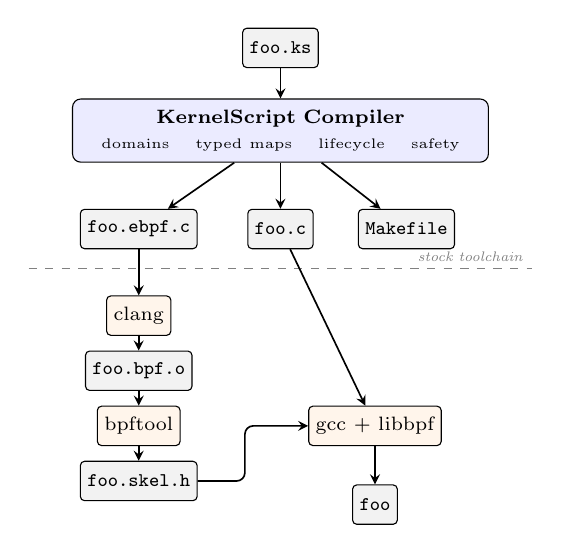
\begin{tikzpicture}[
  font=\scriptsize,
  file/.style={draw, rounded corners=1.5pt, fill=gray!10,
    inner sep=2.5pt, font=\scriptsize\ttfamily, minimum height=5mm},
  phase/.style={draw, rounded corners=3pt, fill=blue!8,
    inner sep=4pt, align=center, text width=50mm},
  tool/.style={draw, rounded corners=1.5pt, fill=orange!8,
    inner sep=2.5pt, minimum height=5mm},
  arr/.style={->, >=stealth, semithick},
]

\node[file] (src) at (0, 0) {foo.ks};

\node[phase] (comp) at (0, -1.05) {%
  \textbf{KernelScript Compiler}\\[1pt]
  {\tiny domains \quad typed maps \quad lifecycle \quad safety}};
\draw[arr] (src) -- (comp);

\node[file] (ebpfc) at (-1.8, -2.3) {foo.ebpf.c};
\node[file] (userc) at (0, -2.3) {foo.c};
\node[file] (makef) at (1.6, -2.3) {Makefile};
\draw[arr] (comp) -- (ebpfc);
\draw[arr] (comp) -- (userc);
\draw[arr] (comp) -- (makef);

\draw[dashed, gray, semithick] (-3.2, -2.8) -- (3.2, -2.8);
\node[anchor=east, gray, font=\tiny\itshape] at (3.2, -2.65) {stock toolchain};

\node[tool] (clang) at (-1.8, -3.4) {clang};
\draw[arr] (ebpfc) -- (clang);

\node[file] (bpfo) at (-1.8, -4.1) {foo.bpf.o};
\draw[arr] (clang) -- (bpfo);

\node[tool] (bpftool) at (-1.8, -4.8) {bpftool};
\draw[arr] (bpfo) -- (bpftool);

\node[file] (skel) at (-1.8, -5.5) {foo.skel.h};
\draw[arr] (bpftool) -- (skel);

\node[tool] (gcc) at (1.2, -4.8) {gcc + libbpf};
\draw[arr] (userc) -- (gcc);
\draw[arr, rounded corners=3pt] (skel.east) -- ++(0.6, 0) |- (gcc.west);

\node[file, font=\scriptsize\ttfamily\bfseries] (bin) at (1.2, -5.8) {foo};
\draw[arr] (gcc) -- (bin);

\end{tikzpicture}
\caption{Compilation pipeline. The compiler checks cross-boundary
invariants and emits C\@; the stock clang/bpftool/libbpf toolchain
produces the final binary.}
\label{fig:pipeline}
\end{figure}

Each typing rule of Section~\ref{sec:model} maps to a concrete compiler pass.
% 第~\ref{sec:model} 节的每条类型规则映射到一个具体的编译器遍。
The compiler attaches a domain to each function as a scope refined by the entry attribute. The IR records each function's program type so that code generation can dispatch the same source function to the eBPF or userspace backend.
% 编译器将域附加到每个函数作为由入口属性细化的作用域。IR 记录每个函数的程序类型，以便代码生成可以将相同的源函数分派到 eBPF 或用户空间后端。
Typed maps lower to a single descriptor that records key and value types once. Both backends read that descriptor to emit the eBPF \code{SEC(".maps")} definition and the userspace accessor (Listing~\ref{lst:map}).
% 类型化映射降低到单个描述符，一次记录键和值类型。两个后端读取该描述符以发出 eBPF \code{SEC(".maps")} 定义和用户空间访问器（清单~\ref{lst:map}）。
Lifecycle handles are enforced in the front end. Only \code{load} yields a \code{ProgramHandle}, and \code{attach} and \code{detach} require one, so a misordered call fails type checking before code generation.
% 生命周期句柄在前端强制执行。只有 \code{load} 产生 \code{ProgramHandle}，而 \code{attach} 和 \code{detach} 需要一个，因此错序调用在代码生成之前类型检查失败。
The handle then lowers to a file descriptor via libbpf APIs.
% 然后句柄通过 libbpf API 降低到文件描述符。

\begin{lstlisting}[language=C,caption={One typed map declaration lowers to both
a kernel \texttt{SEC(".maps")} definition and a userspace accessor from a single
descriptor.},label={lst:map}]
// KernelScript source
var counts : hash<u32, u64>(1024)

// generated eBPF C
struct {
  __uint(type, BPF_MAP_TYPE_HASH);
  __uint(max_entries, 1024);
  __type(key, __u32);
  __type(value, __u64);
} counts SEC(".maps");

// generated userspace C: same key/value types
__u32 key = ...; __u64 val;
bpf_map_lookup_elem(counts_fd, &key, &val);
\end{lstlisting}

The compiler does not replace the verifier, clang, bpftool, or libbpf. Existing diagnostics therefore remain available, and any compatibility failure stays visible.
% 编译器不替换验证器、clang、bpftool 或 libbpf。因此现有诊断保持可用，任何兼容性故障都保持可见。
For interfaces that move faster than the DSL can stabilize, \code{include} and \code{extern} declarations provide a fallback to raw header declarations.
% 对于比 DSL 稳定更快移动的接口，\code{include} 和 \code{extern} 声明提供回退到原始头文件声明。

\section{Evaluation}
\label{sec:eval}

The evaluation answers three questions.
% 评估回答三个问题。
\emph{(Q1)} Does each typed cross-boundary invariant trigger a compile-time diagnostic?
% (Q1) 每个类型化的跨边界不变量是否触发编译时诊断？
\emph{(Q2)} Does a single source generate a complete, buildable libbpf project, and does unifying it reduce maintenance surface?
% (Q2) 单一源是否生成完整的、可构建的 libbpf 项目，统一它是否减少维护表面？
\emph{(Q3)} Does generated code load, attach, and run on a real kernel?
% (Q3) 生成的代码是否在真实内核上加载、附加和运行？
All experiments run on Linux 6.15 with clang 18, bpftool 7.7, and libbpf 1.3.0. SLOC counts exclude blank lines, comments, and generated headers.
% 所有实验在 Linux 6.15 上运行，使用 clang 18、bpftool 7.7 和 libbpf 1.3.0。SLOC 计数排除空行、注释和生成的头文件。

\subsection{Q1: Compile-Time Diagnostic Coverage}

The compiler test suite contains 85 suites and 1095 tests with no failures. These tests cover all major subsystems from lexer to code generation.
% 编译器测试套件包含 85 个套件和 1095 个测试，无失败。这些测试覆盖从词法分析器到代码生成的所有主要子系统。
A separate rejection suite of 28 targeted programs exercises the diagnostics of Section~\ref{sec:model} directly, with one positive control and 27 expected rejections covering lifecycle misuses, program-signature violations, map type errors, domain crossings, and safety violations.
% 另有 28 个目标程序的拒绝套件直接执行第~\ref{sec:model} 节的诊断，包含一个正向控制和 27 个预期拒绝，涵盖生命周期误用、程序签名违规、映射类型错误、域跨越和安全违规。
Each case carries an expected diagnostic substring, so incidental rejections do not count as passing.
% 每个案例都带有预期的诊断子字符串，因此偶然的拒绝不算通过。

To measure whether \tool{} detects mistakes \emph{earlier} than the stock toolchain, we inject four realistic mistakes into a working XDP map-counter in both \tool{} and matched hand-written C/eBPF, recording the earliest rejection stage along a shared ladder (compile $<$ build $<$ verifier $<$ attach $<$ runtime $<$ undetected).
% 为了衡量 \tool{} 是否比原有工具链更早检测到错误，我们向工作中的 XDP 映射计数器注入 4 个现实错误，分别在 \tool{} 和匹配的手写 C/eBPF 中，并沿共享阶梯记录最早的拒绝阶段（编译 $<$ 构建 $<$ 验证器 $<$ 附加 $<$ 运行时 $<$ 未检测）。
As Table~\ref{tab:organic} shows, \tool{} rejects all four at compile time, while C/eBPF ties on all but the cross-boundary case.
% 如表~\ref{tab:organic} 所示，\tool{} 在编译时拒绝所有 4 个错误，而 C/eBPF 除跨边界案例外均打平。
That case passes an \texttt{@xdp} entry point a \texttt{*\_\_sk\_buff} context instead of \texttt{*xdp\_md}. \tool{} rejects it via the program-signature rule of Section~\ref{sec:model}, whereas the C version compiles and loads silently because the body never dereferences the context, giving the verifier no invalid access to flag.
% 该案例向 \texttt{@xdp} 入口点传递 \texttt{*\_\_sk\_buff} 上下文而非 \texttt{*xdp\_md}。\tool{} 通过第~\ref{sec:model} 节的程序签名规则拒绝它，而 C 版本因主体从不解引用上下文而静默编译和加载，验证器没有无效访问可标记。
A body that did read a context field could trip the verifier, though it would report the access violation rather than the underlying context-type confusion.
% 读取上下文字段的主体可能触发验证器，但验证器会报告访问违规而非底层的上下文类型混淆。
The other three mistakes (undeclared map, wrong value type, oversized stack) tie because clang catches them locally.
% 其他 3 个错误（未声明的映射、错误的值类型、超大栈）打平，因为 clang 在本地捕获它们。
Typing therefore helps precisely on cross-boundary relations that local C checking cannot see. Section~\ref{sec:limits} discusses the limits of this author-constructed set.
% 因此类型化恰好帮助本地 C 检查看不到的跨边界关系。第~\ref{sec:limits} 节讨论这个作者构造集合的局限性。

\begin{table}[H]
\centering
\caption{Earliest detection stage per injected mistake (BS = \tool{}). \tool{} is strictly
earlier only on the cross-boundary context-type mistake; the rest are ties
clang already catches.}
\label{tab:organic}
\footnotesize
\begin{tabular}{@{}>{\raggedright\arraybackslash}p{0.24\columnwidth}>{\raggedright\arraybackslash}p{0.24\columnwidth}>{\centering\arraybackslash}p{0.14\columnwidth}>{\centering\arraybackslash}p{0.18\columnwidth}@{}}
\toprule
Injected mistake & Coupling & BS & C/libbpf \\
\midrule
Wrong context type & signature/domain & compile reject & undetected \\
Undeclared map & representation & compile reject & compile reject \\
String into \texttt{u64} value & representation & compile reject & compile reject \\
Oversized stack buffer & safety & compile reject & compile reject \\
\bottomrule
\end{tabular}
\end{table}

\FloatBarrier
\subsection{Q2: Project Generation}

We evaluate 43 \tool{} examples spanning XDP, TC, kprobe, tracepoint, perf\_event, maps, ring buffers, tail calls, kfuncs, and struct\_ops.
% 我们评估了 43 个 \tool{} 示例，涵盖 XDP、TC、kprobe、tracepoint、perf\_event、映射、环形缓冲区、尾调用、kfunc 和 struct\_ops。
For successfully built examples, the compiler emits a median of 472 lines from 31 source lines.
% 对于成功构建的示例，编译器从 31 行源代码发出中位数 472 行。
Across 11 workloads with hand-written C/libbpf baselines, \tool{} sources total 203 lines versus 1105.

Hand-porting three \texttt{xdp-tutorial}~\cite{xdp-tutorial} XDP programs to \tool{} yields comparable line counts to the original C/eBPF.
A source-only scan of three public eBPF repositories confirms that the program types and map patterns we generate (XDP, TC, kprobe, ring buffers, struct\_ops) appear together in real projects.
% 对 3 个公共 eBPF 仓库的纯源代码扫描确认我们生成的程序类型和映射模式（XDP、TC、kprobe、环形缓冲区、struct\_ops）在真实项目中一起出现。

Source-footprint totals measure the size of a finished workload but miss how many places a requirement change must touch.
% 源代码占用空间总计衡量完成的工作负载的大小，但未能反映需求变更时要修改多少位置。
To measure this change-amplification coupling, we construct five matched micro-edits (changing a map from \code{array} to \code{percpu_array}, changing a program from \code{@xdp} to \code{@tc}, moving a \code{perf_event} attach from standalone to grouped, extending a shared ringbuf event schema, and adding ringbuf reporting with userspace handling) and compare diff sizes between \tool{} and hand-written C/libbpf.
% 为了衡量这种变更放大耦合，我们构建 5 个匹配的微编辑（将映射从 array 更改为 percpu\_array，将程序从 @xdp 更改为 @tc，将 perf\_event 附加从独立移至分组，扩展共享 ringbuf 事件模式，以及添加带用户空间处理的 ringbuf 报告）并比较 \tool{} 和手写 C/libbpf 之间的差异大小。
Table~\ref{tab:change-amp} reports file count, edit-site count, changed LOC, and required manual synchronization across kernel code, userspace code, or skeleton/section conventions.
% 表~\ref{tab:change-amp} 报告文件数、编辑位置数、更改的 LOC，以及内核代码、用户空间代码或骨架/节约定之间所需的手动同步。

{\setlength{\intextsep}{4pt}
\begin{table}[H]
\centering
\caption{Change amplification for five matched micro-edits (BS = \tool{}, C = hand-written C/libbpf). ``Sync'' reports
which manually synchronized surfaces change: kernel (K), userspace (U), or
skeleton/section conventions (S).}
\label{tab:change-amp}
\footnotesize
\setlength{\tabcolsep}{4pt}
\renewcommand{\arraystretch}{0.95}
\begin{tabular}{@{}>{\raggedright\arraybackslash}p{0.31\columnwidth}ccccc@{}}
\toprule
Edit & Impl. & Files & Sites & LOC & Sync \\
\midrule
\shortstack[l]{Map \\ \code{array}$\rightarrow$\code{percpu_array}} & BS & 1 & 1 & 2 & --- \\
 & C & 2 & 7 & 19 & K/U/S \\
\addlinespace[2pt]
\shortstack[l]{Program \\ \code{@xdp}$\rightarrow$\code{@tc}} & BS & 1 & 2 & 8 & --- \\
 & C & 2 & 6 & 30 & K/U/S \\
\addlinespace[2pt]
\shortstack[l]{Perf event \\ standalone$\rightarrow$grouped} & BS & 1 & 1 & 6 & --- \\
 & C & 1 & 8 & 91 & U \\
\addlinespace[2pt]
\shortstack[l]{Shared event \\ schema} & BS & 1 & 3 & 4 & --- \\
 & C & 2 & 4 & 7 & K/U \\
\addlinespace[2pt]
\shortstack[l]{Add ringbuf \\ reporting/handling} & BS & 1 & 5 & 23 & --- \\
 & C & 2 & 11 & 89 & K/U/S \\
\bottomrule
\end{tabular}
\end{table}
}

None of the \tool{} edits require manual cross-boundary synchronization, whereas hand-written C/libbpf requires userspace synchronization in 5/5 cases, kernel-side synchronization in 4/5, and skeleton or section-convention synchronization in 3/5.
% \tool{} 的编辑都不需要手动跨边界同步，而手写 C/libbpf 在 5/5 个案例中需要用户空间同步，在 4/5 个案例中需要内核侧同步，在 3/5 个案例中需要骨架或节约定同步。
Diff-size medians reinforce this: \tool{} touches 1 file, 2 edit sites, and 6 lines, versus 2, 7, and 30 for C/libbpf.
% 差异大小中位数强化了这一点：\tool{} 触及 1 个文件、2 个编辑位置和 6 行，而 C/libbpf 为 2、7 和 30。
With only five edits these numbers are illustrative, but they show that a unified typed source reduces change amplification beyond total line count.
As cross-boundary structure accumulates (pass-only XDP → counter map → ring-buffer reporting), \tool{} grows more slowly: +2 lines for the counter map versus +11 in C/libbpf, and +12 for ring-buffer reporting versus +202.
By the reporting stage, C/libbpf reaches 9$\times$ the \tool{} source size.
% 在两种情况下，DSL 扩展一个文件，而 C/libbpf 在内核和用户空间表面累积协调代码。

\subsection{Q3: Runtime Validation}
\label{sec:eval:q3}

On a real kernel, 27 XDP examples attach and detach successfully. Additional workloads exercise TC and struct\_ops.
% 在真实内核上，27 个 XDP 示例都成功附加和分离。额外的工作负载执行 TC 和 struct\_ops。

Matched workloads confirm the generated objects run correctly.
% 匹配的工作负载确认生成的对象正确运行。
Under \code{BPF_PROG_TEST_RUN}, a minimal generated XDP pass program matches its hand-written baseline in instruction count and latency. Over ten veth/iperf3 trials, both generated and hand-written XDP and TC programs deliver comparable throughput.
% 在 BPF\_PROG\_TEST\_RUN 下，最小生成的 XDP 通过程序在指令数和延迟方面与其手写基线匹配。在 10 次 veth/iperf3 试验中，生成的和手写的 XDP 及 TC 程序都提供相当的吞吐量。
These numbers are sanity checks for functional equivalence, not performance claims.
% 这些数字是功能等价的健全性检查，而不是性能声明。

\section{Limitations}
\label{sec:limits}

The differential probe injects four hand-chosen mistakes rather than bugs mined from revision histories.
% 更强的研究将从修订历史中挖掘真实的 eBPF 错误。
Lifecycle typing enforces a producer/consumer handle distinction without full typestate. Use-after-detach and leaked handles therefore remain possible.
% 生命周期类型化强制生产者/消费者句柄区分而没有完整的类型状态。因此分离后使用和泄漏的句柄仍然可能。
The example programs are author-written. The external port shows that line-count savings vary when porting existing code rather than writing from scratch.
% 示例程序由作者编写。外部移植表明当移植现有代码而非从头编写时，行数节省有所不同。
The change-amplification study uses small checked-in micro-edits instead of real revision histories. It measures maintenance-surface coupling, not actual developer time or debugging effort.
% 变更放大研究使用小的签入微编辑而非真实的修订历史。因此它衡量维护表面耦合，而非真正的开发者时间或调试工作。
Traffic numbers are local sanity checks, not performance claims.
% 流量数字是本地健全性检查，而不是性能声明。

\section{Related Work}

Prior work on eBPF development falls into three categories.
% 关于 eBPF 开发的先前工作分为三类。
Domain-specific DSLs target particular use cases: bpftrace for tracing~\cite{bpftrace}, BPFBox and ActPlane for policy enforcement~\cite{bpfbox,actplane}, BMC for caching~\cite{bmc}, P4c-eBPF for networking~\cite{p4c-ebpf}, and Yaksha-Prashna for bytecode analysis~\cite{yaksha}.
% 领域特定 DSL 针对特定用例：用于追踪的 bpftrace、用于策略执行的 BPFBox 和 ActPlane、用于缓存的 BMC、用于网络的 P4c-eBPF，以及用于字节码分析的 Yaksha-Prashna。
These DSLs primarily target kernel-side code and do not type the full cross-boundary structure that \tool{} addresses.
% 这些 DSL 主要针对内核侧代码，不对 \tool{} 所处理的完整跨边界结构进行类型化。
General eBPF development tools include the standard eBPF development workflow~\cite{libbpf}, Aya for Rust~\cite{aya}, Rex for safe Rust kernel extensions without a verifier~\cite{rex}, Wasm-bpf for WebAssembly deployment~\cite{wasmbpf}, and eunomia-bpf for dynamic loading~\cite{eunomia-bpf}.
% 通用 eBPF 开発工具包括标准 eBPF 开发工作流、用于 Rust 的 Aya、不使用验证器的安全 Rust 内核扩展 Rex、用于 WebAssembly 部署的 Wasm-bpf，以及用于动态加载的 eunomia-bpf。
These reduce boilerplate but leave lifecycle and representation relationships implicit.
% 这些减少样板但使生命周期和表示关系保持隐式。
Verified approaches take a different direction: BeePL provides correct-by-compilation kernel extensions~\cite{beepl}, and Jitk and Serval verify JIT correctness~\cite{jitk,serval}.
% 验证方法采取不同方向：BeePL 提供编译即正确的内核扩展，Jitk 和 Serval 验证 JIT 正确性。
\tool{} occupies a middle ground. It generates both kernel and userspace code from one source and types cross-boundary relationships. The goal is practical integration with the existing toolchain, not formal verification.
% \tool{} 占据中间地带。它从一个源生成内核和用户空间代码并对跨边界关系进行类型化。目标是与现有工具链的实际集成，而非正式验证。

\section{Conclusion}

\tool{} treats the cross-boundary structure of an eBPF application (program lifecycle, shared maps, and execution domains) as something a compiler can type, replacing conventions and late verifier/attach-time discovery.
% \tool{} 将 eBPF 应用程序的跨边界结构（程序生命周期、共享映射和执行域）视为编译器可以类型化的东西，取代约定和延迟的验证器/附加时发现。
The evaluation confirms that each typed invariant triggers a compile-time diagnostic, that a single source generates buildable libbpf projects, and that generated objects load, attach, and pass traffic on a real kernel.
% 评估确认每个类型化的不变量触发编译时诊断，单一源生成可构建的 libbpf 项目，生成的对象在真实内核上加载、附加并传递流量。
The result is a concrete design point: typing eBPF's cross-boundary structure is feasible.
% 结果是一个具体的设计点：对 eBPF 的跨边界结构进行类型化是可行的。
Because the compiler lowers through the stock toolchain, the type system's guarantees and the version-skew limits it cannot absorb both remain visible and measurable.
% 因为编译器通过原有工具链降低，类型系统的保证和它无法吸收的版本偏差限制都保持可见和可测量。

\newpage
\bibliographystyle{ACM-Reference-Format}
\bibliography{references}

\end{document}
